\section{Pengujian \& Evaluasi}

\subsection{Kecepatan Sistem}
Pengujian kecepatan dilakukan dengan menggunakan Google Chrome Developer Tools, dimana untuk setiap kasus penggunaan diuji dengan segmentasi \textit{loading time} sebagai berikut \begin{inlinelist}
	\item \textit{DOM Loading}
	\item \textit{Scripting}
	\item \textit{Rendering}
\end{inlinelist}. Rata-rata keseluruhan \textit{loading page} adalah 3,2 detik (lebih 6\% dari target). Untuk menganalisa dengan visualisasi masing-masing segmen pada Gambar \ref{bar-chart-speed}.
\begin{figure}[b]
	\centering
	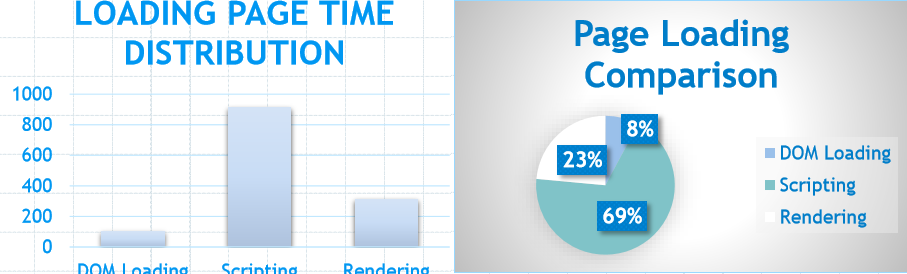
\includegraphics[width=.4\textwidth]{images/bab5/speed/combined.png}
	\caption{Diagram Visualisasi dan Perbandingan Waktu per Segmen}
	\label{bar-chart-speed}
\end{figure}
	Dengan menggunakan \textit{tool} Lighthouse, \textit{scripting} memakan waktu yang sangat besar (hampir 75|\% \textit{loading time}) untuk \textit{loading} gambar, yang ternyata ini menjadi masalah umum pada website \textit{e-commerce}, dimana penyelesaiannya menggunakan teknik \textit{image optimization}.

\subsection{\textit{Maintainability Assesment}}
Pengujian \textit{maintainability} dilakukan dengan mengikuti pedoman dari paper "A Software Maintainability Evaluation Methodology"\cite{peercy_software_nodate}, yaitu parameter utama: \textit{modularity}, \textit{descriptiveness}, \textit{consistency}, \textit{simplicity}, dan \textit{trackability}. Sesuai dengan paper tersebut, dengan dua aspek penilaian - kode sumber dan dokumentasi sistem dengan \textit{weight} masing-masing yang berbeda - rekapitulasi hasil dapat dilihat pada Gambar \ref{maintainability-recap}.

\begin{table}[h]
	\centering
	\caption{Rekapitulasi Pengujian \textit{Maintainability Assesment}}
	\label{maintainability-recap}
	\begin{tabular}{c|c|c|c}
		\toprule
		\textbf{Parameter} & \textbf{Kode Sumber} & \textbf{Dokumentasi Sistem} & \textbf{Rata-rata} \\
		\hline
		
		\textit{Modularity} & 83\% & 83\% & 83\% \\ 
		\textit{Descriptiveness} & 83\% & 78\% & 80\% \\ 
		\textit{Consistency} & 78\% & 73\% & 75\% \\ 
		\textit{Simplicity} & 75\% & 73\% & 74\% \\ 
		\textit{Trackability} & 75\% & 73\% & 77\% \\ 
		Rata-rata & 79\% & 76\% &  \\ 
		\textit{weight} & 0.6 & 0.4 &  \\ \hline
		\textbf{Skor} & \multicolumn{3}{|c}{77\% (pencapaian 96\%)} \\ \hline
	\end{tabular}
\end{table}

\subsection{\textit{User Experience Assesment}}
Pengujian \textit{maintainability} dilakukan dengan mengikuti pedoman dari paper " Development of an Instrument Measuring User Satisfaction of the Human-Computer Interface"\cite{chin_development_1998}. Rekapitulasi hasil dapat dilihat pada Tabel \ref{ux-recap}, dan visualisasi hasil berbentuk diagram dapat dilihat pada Gambar \ref{ux-chart}.

\begin{table}[t]
	\centering
	\caption{Rekapitulasi Hasil \textit{User Experience Assesment}}
	\label{ux-recap}
	\vfill
	\begin{tabular}{c|c|c|c}
		\hline
		\toprule
		\textbf{\begin{tabular}[c]{@{}c@{}}Parameter/\\ Kriteria\end{tabular}} & \textbf{\begin{tabular}[c]{@{}c@{}}Skor\\ Aplikasi Lain\end{tabular}} & \textbf{\begin{tabular}[c]{@{}c@{}}Skor\\ Aplikasi Lelangapa\end{tabular}} & \textbf{\begin{tabular}[c]{@{}c@{}}Persentase\\ Perbedaan\end{tabular}} \\ \hline
		
		\midrule
		
		\begin{tabular}[c]{@{}c@{}}Desain\\ \& Impresi Web\end{tabular} & 3.3 & 4.1 & +20\% \\ 
		\begin{tabular}[c]{@{}c@{}}Konsistensi\\ \& Descriptiveness\end{tabular} & 3.5 & 4.2 & +17\% \\ 
		\textit{Easiness} & 3.1 & 3.9 & +21\% \\ 
		\textit{\begin{tabular}[c]{@{}c@{}}Clear \\ Error Messages\end{tabular}} & 3.7 & 3.9 & +5\% \\ 
		\textit{\begin{tabular}[c]{@{}c@{}}Clear\\ Status Process\end{tabular}} & 3.3 & 4 & +18\% \\ 
		\textit{Performance} & 3.7 & 3.8 & +3\% \\ 
		\begin{tabular}[c]{@{}c@{}}Penilaian\\ Keseluruhan\end{tabular} & 3.7 & 4.3 & +14\% \\ 
		\begin{tabular}[c]{@{}c@{}}Rekomendasi\\ pada Teman?\end{tabular} & 3.4 & 4.0 & +15\% \\ \hline
		\multicolumn{3}{c}{\textbf{Total Rata-rata Keseluruhan}} & \multicolumn{1}{c}{+15\%} \\ 
		
		\bottomrule
	\end{tabular}
\end{table}

\begin{figure}[b]
	\centering
	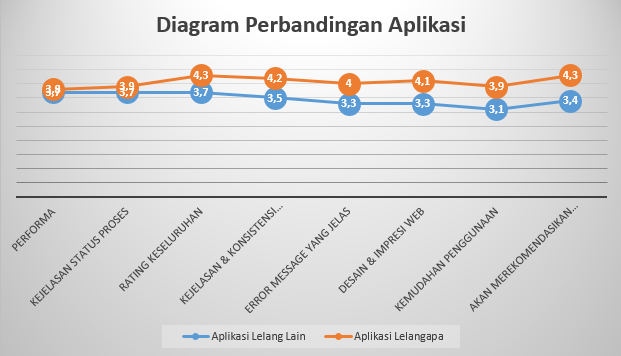
\includegraphics[width=.4\textwidth]{images/bab5/ujipengguna/chart.png}
	\caption{Visualisasi Perbandingan Hasil \textit{User Experience Assesment} Aplikasi dengan Aplikasi Lainnya}
	\label{ux-chart}
\end{figure}


